\documentclass[tikz]{standalone}
\usepackage{tikz-feynman}
\begin{document}
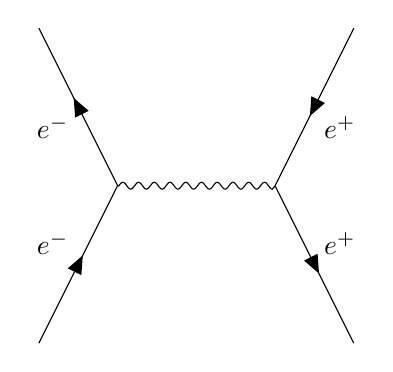
\begin{tikzpicture}
\begin{feynman}
\vertex(q);
\vertex[above=4cm of q](q1);
\vertex[right=4cm of q](q4);
\vertex[right=4cm of q1](q5);
\vertex[right=1 cm  of q](iq);
\vertex[above= 2cm of iq](q2);
\vertex[right = 2cm of q2](q3);
\diagram*{
(q)--[fermion, edge label=$e^-$](q2)--[fermion, edge label=$e^-$](q1);
(q5)--[fermion, edge label=$e^+$](q3)--[fermion, edge label=$e^+$](q4);
(q2)--[photon](q3);
};
\end{feynman}
\end{tikzpicture}  %original and rotation by 180
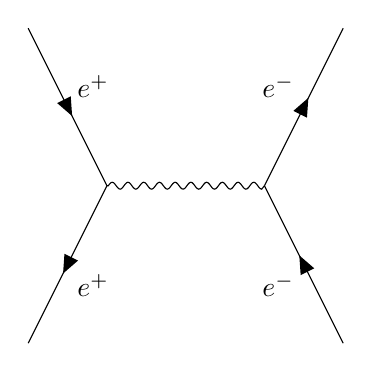
\begin{tikzpicture}
\begin{feynman}
\vertex(q);
\vertex[above=4cm of q](q1);
\vertex[right=4cm of q](q4);
\vertex[right=4cm of q1](q5);
\vertex[right=1 cm  of q](iq);
\vertex[above= 2cm of iq](q2);
\vertex[right = 2cm of q2](q3);
\diagram*{
(q4)--[fermion, edge label=$e^-$](q3)--[fermion, edge label=$e^-$](q5);
(q1)--[fermion, edge label=$e^+$](q2)--[fermion, edge label=$e^+$](q);
(q2)--[photon](q3);
};
\end{feynman}
\end{tikzpicture} %mirror and mirror + 180 rot
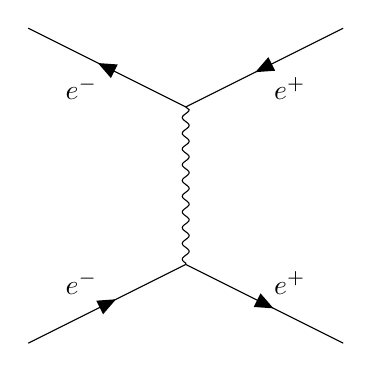
\begin{tikzpicture}
\begin{feynman}
\vertex(q);
\vertex[right=4cm of q](q1);
\vertex[above=4cm of q](q4);
\vertex[above=4cm of q1](q5);
\vertex[above=1 cm  of q](iq);
\vertex[right= 2cm of iq](q2);
\vertex[above = 2cm of q2](q3);
\diagram*{
(q)--[fermion, edge label=$e^-$](q2)--[fermion, edge label=$e^+$](q1);
(q5)--[fermion, edge label=$e^+$](q3)--[fermion, edge label=$e^-$](q4);
(q2)--[photon](q3);
};
\end{feynman}
\end{tikzpicture} %mirror+90/270 degree rot

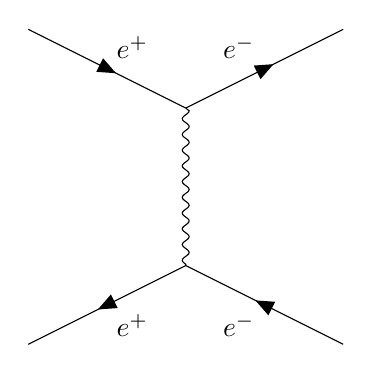
\begin{tikzpicture}
\begin{feynman}
\vertex(q);
\vertex[right=4cm of q](q1);
\vertex[above=4cm of q](q4);
\vertex[above=4cm of q1](q5);
\vertex[above=1 cm  of q](iq);
\vertex[right= 2cm of iq](q2);
\vertex[above = 2cm of q2](q3);
\diagram*{
(q1)--[fermion, edge label=$e^-$](q2)--[fermion, edge label=$e^+$](q);
(q4)--[fermion, edge label=$e^+$](q3)--[fermion, edge label=$e^-$](q5);
(q2)--[photon](q3);
};
\end{feynman}%90, 270 degree rot
\end{tikzpicture}
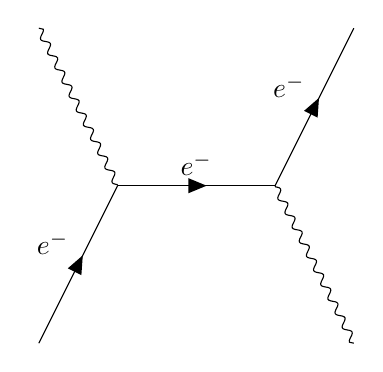
\begin{tikzpicture}
\begin{feynman}
\vertex(q);
\vertex[above=4cm of q](q1);
\vertex[right=4cm of q](q4);
\vertex[right=4cm of q1](q5);
\vertex[right=1 cm  of q](iq);
\vertex[above= 2cm of iq](q2);
\vertex[right = 2cm of q2](q3);
\diagram*{
(q)--[fermion, edge label=$e^-$](q2)--[photon](q1);
(q3)--[fermion, edge label=$e^-$](q5);
(q3)--[photon](q4);
(q2)--[fermion, edge label=$e^-$](q3);
};
\end{feynman}
\end{tikzpicture} %base for rows
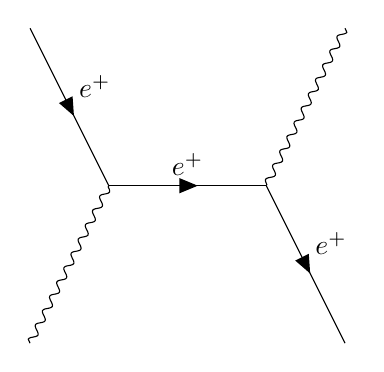
\begin{tikzpicture}
\begin{feynman}
\vertex(q);
\vertex[above=4cm of q](q1);
\vertex[right=4cm of q](q4);
\vertex[right=4cm of q1](q5);
\vertex[right=1 cm  of q](iq);
\vertex[above= 2cm of iq](q2);
\vertex[right = 2cm of q2](q3);
\diagram*{
(q1)--[fermion, edge label=$e^+$](q2)--[photon](q);
(q3)--[fermion, edge label=$e^+$](q4);
(q3)--[photon](q5);
(q2)--[fermion, edge label=$e^+$](q3);
};
\end{feynman}
\end{tikzpicture} %rot of 180
\begin{tikzpicture}
\begin{feynman}
\vertex(q);
\vertex[above=4cm of q](q1);
\vertex[right=4cm of q](q4);
\vertex[right=4cm of q1](q5);
\vertex[right=1 cm  of q](iq);
\vertex[above= 2cm of iq](q2);
\vertex[right = 2cm of q2](q3);
\diagram*{
(q)--[fermion, edge label=$e^-$](q2)--[photon](q1);
(q3)--[fermion, edge label=$e^+$](q4);
(q3)--[photon](q5);
(q2)--[fermion, edge label=$e^-$](q3);
};
\end{feynman}
\end{tikzpicture} %second basis
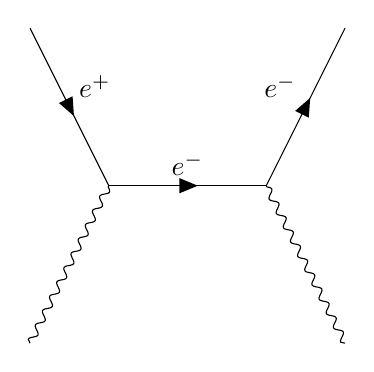
\begin{tikzpicture}
\begin{feynman}
\vertex(q);
\vertex[above=4cm of q](q1);
\vertex[right=4cm of q](q4);
\vertex[right=4cm of q1](q5);
\vertex[right=1 cm  of q](iq);
\vertex[above= 2cm of iq](q2);
\vertex[right = 2cm of q2](q3);
\diagram*{
(q1)--[fermion, edge label=$e^+$](q2)--[photon](q);
(q3)--[fermion, edge label=$e^-$](q5);
(q3)--[photon](q4);
(q2)--[fermion, edge label=$e^-$](q3);
};
\end{feynman} %rot of 180
\end{tikzpicture}

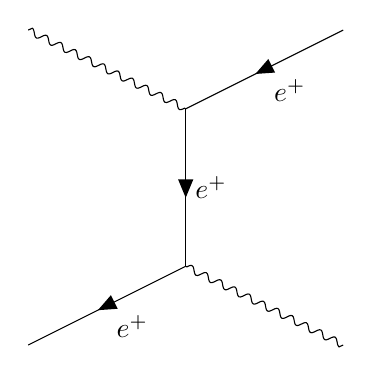
\begin{tikzpicture}
\begin{feynman}
\vertex(q);
\vertex[right=4cm of q](q1);
\vertex[above=4cm of q](q4);
\vertex[above=4cm of q1](q5);
\vertex[above=1 cm  of q](iq);
\vertex[right= 2cm of iq](q2);
\vertex[above= 2cm of q2](q3);
\diagram*{
(q2)--[fermion, edge label=$e^+$](q);
(q2)--[photon](q1);
(q5)--[fermion, edge label=$e^+$](q3);
(q3)--[photon](q4);
(q3)--[fermion, edge label=$e^+$](q2);
};
\end{feynman}
\end{tikzpicture} %base for rows
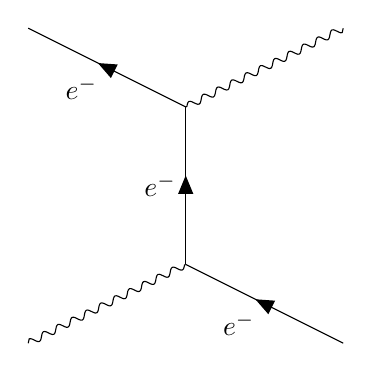
\begin{tikzpicture}
\begin{feynman}
\vertex(q);
\vertex[right=4cm of q](q1);
\vertex[above=4cm of q](q4);
\vertex[above=4cm of q1](q5);
\vertex[above=1 cm  of q](iq);
\vertex[right= 2cm of iq](q2);
\vertex[above= 2cm of q2](q3);
\diagram*{
(q1)--[fermion, edge label=$e^-$](q2)--[photon](q);
(q3)--[fermion, edge label=$e^-$](q4);
(q3)--[photon](q5);
(q2)--[fermion, edge label=$e^-$](q3);
};
\end{feynman}
\end{tikzpicture} %rot of 180
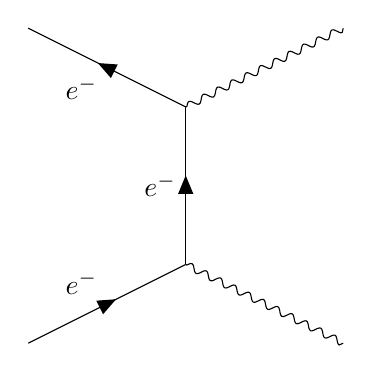
\begin{tikzpicture}
\begin{feynman}
\vertex(q);
\vertex[right=4cm of q](q1);
\vertex[above=4cm of q](q4);
\vertex[above=4cm of q1](q5);
\vertex[above=1 cm  of q](iq);
\vertex[right= 2cm of iq](q2);
\vertex[above= 2cm of q2](q3);
\diagram*{
(q)--[fermion, edge label=$e^-$](q2)--[photon](q1);
(q3)--[fermion, edge label=$e^-$](q4);
(q3)--[photon](q5);
(q2)--[fermion, edge label=$e^-$](q3);
};
\end{feynman}
\end{tikzpicture} %second basis
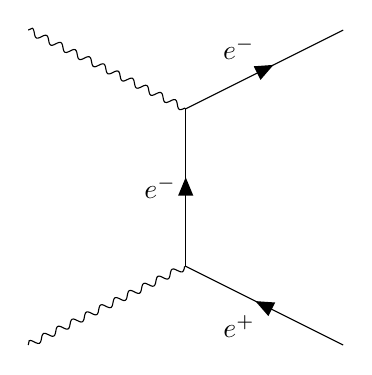
\begin{tikzpicture}
\begin{feynman}
\vertex(q);
\vertex[right=4cm of q](q1);
\vertex[above=4cm of q](q4);
\vertex[above=4cm of q1](q5);
\vertex[above=1 cm  of q](iq);
\vertex[right= 2cm of iq](q2);
\vertex[above= 2cm of q2](q3);
\diagram*{
(q1)--[fermion, edge label=$e^+$](q2)--[photon](q);
(q3)--[fermion, edge label=$e^-$](q5);
(q3)--[photon](q4);
(q2)--[fermion, edge label=$e^-$](q3);
};
\end{feynman} %rot of 180
\end{tikzpicture}
\end{document}